\chapter{Introduction}
\label{Introduction}
The purpose of user involvement in the design process of any given product is to develop a product that's easy to interact with for the regular user. A common problem with having engineers design these products is that they are experts in technology but are limited in their understanding of people. As a result the final product may be designed logically according to their understanding but may not match the understanding of the users \parencite[][6]{PDF:DonNorman}. User experience designers (UX) intend to counter this issue as full members of the design process by applying knowledge of the users, providing more relevant and meaningful experiences for them \parencite{WEB:UXDesign}. However, there still seems to be some misconception to this among classical engineers, both from a simple web search of the vast amount of forums covering UX and from personal experience. This chapter will therefore start with an interpretation of user involvement in the design process with regards to the terms \textit{user experience design} and \textit{usability} before moving on to the scope of this project.

\section{The benefits of user centered design}
\label{UXbenefits}
The term \textit{user experience} was originally coined by Don Norman in 1993 while working at apple. He defined it as everything that touches upon the user's experience with the product from first acquiring it to actually interacting with it and later evaluating this experience \parencite{WEB:DonNormanOnUX}. Numerous interpretations have since been formulated with $allaboutux.org$ containing a vast amount of these. Despite the differences in phrasing, what seems to be a common trait for these is that UX should be considered a broader term also covering other terms such as usability \parencite{WEB:UXDefinitions}. By investigating an ISO standard on human-centered design for interactive systems, this is emphazised, as UX is defined as \textit{a person's perceptions and responses resulting from the use and/or anticipated use of a product, system or service}. Three notes further elaborates how this includes all aspects of the person's emotions, beliefs, preferences, etc. \parencite[][3]{WEB:UXISO}. In the same ISO standard, usability is defined as \textit{the extend to which a product can be used by specified goals with effectiveness, efficiency and satisfaction in a specified context.} \parencite{WEB:UXISO}. These standards support that UX is the broader term to other terms as usability.\\

\noindent
Designing with a user-centered approach holds multiple benefits. \textcite{WEB:UXBenefits} describes these with regards to both the benefits for the users but also for the design process in general and the members. For example, by having UX designers in the design team they can first of all apply the necessary understanding of users that classical engineers don't possess, as previously mentioned. By understanding the users, the UX designers will then be able to understand the problems they may face by observing the way they interact with the system in question. Secondly, sales increase when products satisfies users. Designers develop products from their own mental model of how they think the product should look, and how it should behave. The designers expect the users to have an identical model to them, but since the user typically can't speak with the designer, the burden of communicating this model lies solely on the product itself including documentations and manuals \parencite[][31]{PDF:DonNorman}. If it isn't clear to the users how they interact with the product, they won't have a satisfying experience with it. However, if the appropriate information is available to make the product understandable and usable, especially in situations when things go wrong and needs to be corrected, then the user is more likely to have a pleasent experience \parencite[][32]{PDF:DonNorman}. Finally the design team itself can also benefit from the involvement of a UX designer. The better understanding of the users' needs the design team have, the better their basis is for estimating the required amount of time and money for both development and subsequent maintenance of the product \parencite{WEB:UXBenefits}.\\

\noindent
Despite the outlined benefits of a user-centered approach to the design process, it is not yet fully integrated in the industry, and the reason for this lies in the difference of how the academic world develops methods for UX and usability testing, and how the industry utilizes these. Dennis Wixon stated in 2003 that \textit{"The literature evaluating usability methods is fundamentally flawed by its lack of relevance to applied usability work"} \parencite{WEB:WixonUXindustry}, this supports the concept of a gap between academia and industry. Several studies have since been made on this with \textcite{WEB:TinaOgLarsBo} being of interest. The purpose of this study was to investigate how 8 different companies changed how they worked within the fields of UX and usability over a period of 2 years. Interviews were held in 2013 and 2015 to uncover a positive development in the companies' understanding of UX and usability during these two years. Almost all of the companies had developed or were developing ways of implementing UX in their design process with examples such as low-fi prototyping, usability testing, workshops, personas, expert evaluations, etc. \parencite[][48]{WEB:TinaOgLarsBo}. in correlation with this, it is important to emphasize that almost all of these companies follows the agile \textit{Scrum} framework in their design process, which means that development is carried out as an iterative process in the form of sprints with the option of going back and making changes to the product in between these.

More papers have recently been released on this topic and the challenges facing it. In a paper by \textcite{PDF:EvolutionofagileUXD}, the focus is on analyzing the evolution and current state of agile UX to provide a brief overview of theses challenges yet to be solved. It also takes its starting point in the increasing attention UX has gotten in the last 16 years, as designers and developers do understand the importance of each others work but don't know how to synchronize their daily operations in a meaningful way. As previously mentioned, the challenge lies in making UX relevant to the specific work in focus, but the challenge also lies in making everyone in the design team understand UX as a team discipline rather than a role in the team. As such, a more thorough understanding of UX and the agile framework is required to help both fields reach a shared understanding of  each other \parencite[][2]{PDF:EvolutionofagileUXD}. For \textcite{WEB:AgilityForUX} the focus is specifically on how UX and agility contribute to each other. The notion is that what helps a software developer to be agile may not help a UX consultant to be agile in the same way and vice versa. This is already well addressed as true, and the findings presented in the study further supports this notion. The study was conducted in an unspecified danish software company with \textit{Conboy's theory of agility} as research approach, which is elaborated on in the paper \parencite[][3]{WEB:AgilityForUX}. The study showed that the two practices contributed substantially different to agility for UX consultants and developers in correlation with different aspects of the design process. Finally, by consulting Nielsen Norman Group it is clear that despite the tendency of UX professionals perceiving Scrum meetings as barriers to productivity, they should still be involved in these meetings to stay engaged and aware of what's going on in the team \parencite{WEB:UXResponsibilitiesInScrum}. It proposes that UX should take part in the scrum framework equivalently to any other member of the design team. This includes daily meetings addressing the questions \textit{what did you do yesterday?} \textit{what will you do today?} and \textit{what is in your way?} This is considered important, as UX designers usually are working ahead of the engineering team on how the product should be shaped. Furthermore, the UX designers should also engage in the work of the other members of the team, as UX designers may be able to help resolve potential issues they may face.


\section{Focus of the project}
\label{ProjectFocus}
It is by now well addressed, that user involvement is a growing trend in software companies, and has been in the last 16 years, whether it is in the form of UX or usability testing. This project intends to investigate this topic of user involvement in the industry in collaboration with a danish company interested in employing these approaches, TC Electronic.\\

\noindent
\textbf{TC Electronic} is a worldwide known manufacturer of effect units for guitarists, originally formed in the early 1970's by Kim and John Rishøj in Aarhus, Denmark. Besides effect units, they also develop other audio equipment such as amplifiers, sound and picture production systems, and broadcast systems \parencite{WEB:TCElectronic}. The project group has worked with TC electronic in previous studies and as such knows that they don't have a dedicated strategy for implementing UX in their design process, but they are interested in implementing it in their existing organization.\\

\noindent
The collaboration was agreed upon through dialogue with TC Electronic themselves, as they are frequent producers of project proposals for Engineering Psychology. After some mail correspondence and a meeting at their headquarters, a scope for the project was agreed upon. It's of interest for TC Electronic to explore the application of user involvement in the design of a future product related to their popular TonePrint pedals, which will be elaborated on in the next section.

\subsection{The Scrum framework}
\label{scrum}
As previously stated, much of the problem with employing a proper UX strategy in software development companies is due to UX not reconciling well with the agile scrum framework. The development teams of TC Electronic also employs this framework, and as such it seems fit to provide a proper description of it.

The scrum framework has gained popularity in the industry of developing software and hardware, as it has contributed to faster market times, greater flexibility, higher-quality products, and customer satisfaction \parencite[][40]{PDF:Scrum}. The overall concept is that the work is split into development iterations referred to as \textit{sprints}. These periods are typically of one month or less where a clear objective is set up and carried out by the \textit{Scrum team} which consists of the members of the development team. There are three different roles for the members, each expected to be self-organizing and cross-functional without being dependent on others outside the team \parencite[][41]{PDF:Scrum}.
%
\begin{itemize}
	\item \textbf{The Scrum Master} serves, much as the name indicates, as the leader of the Scrum Team. His primary objective is to make sure that the work to be done is understood and carried out by the Scrum Team.
	\item \textbf{The Product Owner} focuses on maximizing the work of the development team. He manages the list of requirements that the end product must meet, also known as the \textit{The Product Backlog}. This includes defining the backlog items and prioritizing them in order to optimize the value of the work done by the development team
	\item \textbf{The Development Team} consists of the remaining members of the Scrum Team, which typically is three professionals. Their goal is to execute the objectives established by The Product Owner and Scrum Master, and have them done by the end of sprint. 
\end{itemize}
%
The sprint starts with the initial planning by the members of the scrum team. During this phase they determine realistic goals for the sprint in correlation with what they want to achieve. The steps required to achieve their goals for the sprint are then determined from the backlog items as well through discussions with the product owner. When this is settled, the sprint starts. During the sprint, the team sets aside 15 minutes every day in order to synchronize activities and develop a plan for the next 24 hours. this is simply referred to as \textit{The Daily Scrum} \parencite[][41]{PDF:Scrum}. By the end of the sprint, the period is reviewed by the team in order to evaluate what has been achieved during the sprint, and what still needs to be done in order to complete the current sprint within the assigned time frame. Finally, a retrospective meeting inspects the sprint in order to discuss possible improvements for the next sprint to come. \autoref{fig:ScrumExplanation} provides a graphical elaboration of this process.

%
\begin{figure}[H]
	\centering
	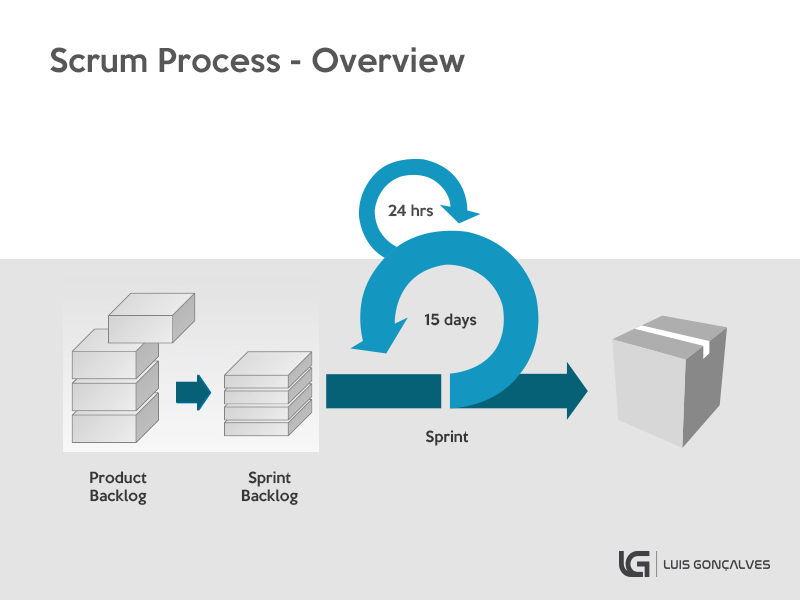
\includegraphics[width=\textwidth]{SCRUM.png}
	\caption{a graphical overview of the Scrum Process. \url{https://luis-goncalves.com/what-is-scrum-methodology/}}
	\label{fig:ScrumExplanation}
\end{figure}
%

\section{The TonePrint concept}
\label{TonePrintConceptDefined}
Effect pedals in general are well known units for guitarists and bassists alike, spanding multiple music genres. The pedal works by taking the input signal from the guitar and changing it to the tweaking by the users. Depending on the effect type, and when playing, the user activates these changes by a single button on the pedal. An example of a simple guitar effect pedal is displayed on \autoref{fig:EffectPedalExample}, where the adjustable parameters on it consists of \textit{Dwell, Mix,} and \textit{Tone}. Each of these are accessed and tweaked with individual knobs on the unit, which gives the user a limited range of ways to change the sound. With this limitation as a motivation, TC created the TonePrint concept, enabling users to tweak the sound of effects beyond the parameters on the pedals. Using the TonePrint application, the users have a vast selection of custom presets with further parameters available for tweaking. These presets are what the term \textit{TonePrint} covers and they are either created in collaboration with professional musicians or by the common user. In order to distinguish these from each other, they are referred to as \textit{Artist TonePrints} and \textit{User TonePrints} respectively. After selecting one for the effect pedal in question, the user can make any desired tweaking or transfer it directly to the pedal with the option of altering it even more on the physical knobs \parencite{PDF:TonePrintAnalyse}. TC has collaborated with multiple guitarists and bassists, creating TonePrints for effect pedals used by the artists themselves. After the creators are satisfied with their TonePrints, they are uploaded to the TonePrint library in the application where any users of the same effect pedal can download the TonePrint and as such match the sound of their favourite artist. For User TonePrints the overall concept is the same. They differ in the fact that the creator isn't a famous guitarist, but the TonePrint is still made using the application and can be transferred directly to its effect pedal. However, when it comes to sharing these User TonePrint with friends and other aspiring guitarist, a platform for this purpose doesn't exist yet.
%
\begin{figure}[H]
	\centering
	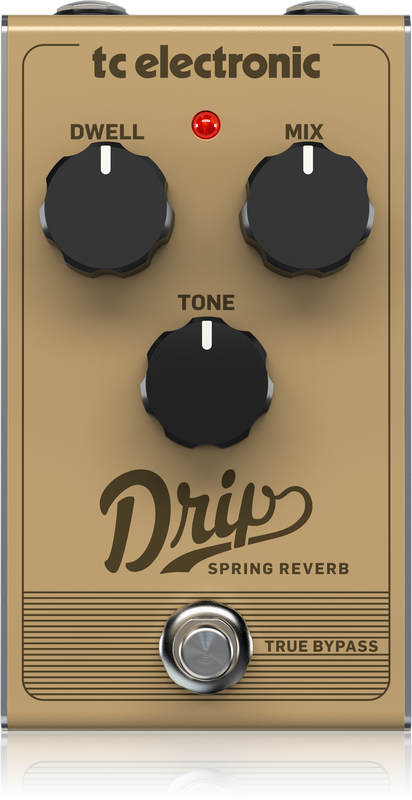
\includegraphics[width=.20\textwidth]{Graphics/EffectPedalExample}
	 \caption{This figure shows a Drip spring reverb effect pedal by TC Electronic \url{https://www.tcelectronic.com/Categories/Tcelectronic/Guitar/Stompboxes/DRIP-SPRING-REVERB/p/P0CQ2\#googtrans(en|en)}.}
    \label{fig:EffectPedalExample}
\end{figure}
%
\subsection{The TonePrint Software}
\label{TonePrintSoftware}
As previously stated, the exploring of TonePrints start with the TonePrint application available for smartphones and tablets. However, the software is also available for PC and MAC, and the reason for this distinction lies in the difference of how a TonePrint is transferred to its respective pedal. For PC and MAC the user is required to use a cable from the computer to the pedal, but through the tablet and smartphone application, the user also have the option of beaming it directly to the pedal. whatever the platform, however, when opening the software the user is introduced to a list selection of different effect pedals, each holding a vast number of TonePrints created by famous guitarists. After selecting an effect pedal from this list, the user is then presented a new list selection of the many guitarist who have created TonePrints for this pedal. When selecting one of the guitarists, and depending on whether the guitarist have created more TonePrints for the same pedal, the user is then presented a bigger view of this specific TonePrint with a description of it and its creator. An example of this is displayed on \autoref{fig:TonePrintAppExample}. Depending on the users' motivation when opening the application first time, they can also choose to browse by artist instead of pedal, if their starting point is to find out what it takes to sound like their favourite artist.

\begin{figure}[H]
	\centering
	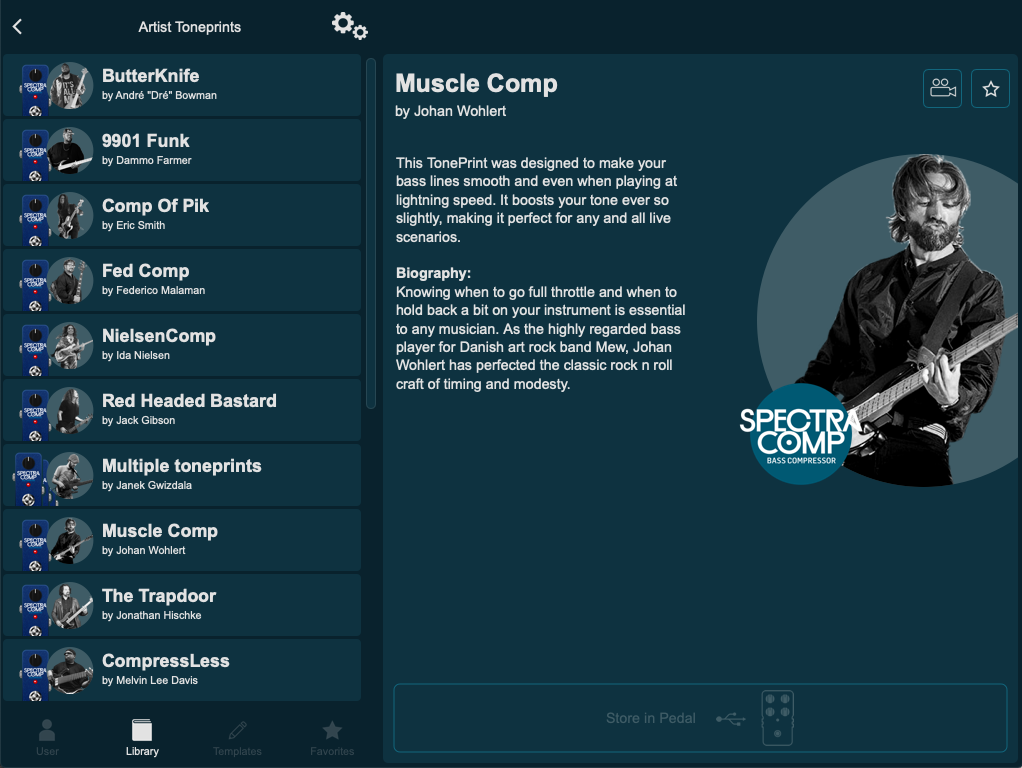
\includegraphics[width=\textwidth]{TonePrintAppExample}
	\caption{The view in the TonePrint application after selecting an effect pedal and a TonePrint. This example displays a TonePrint created by Johan Wohlert of the danish rock band \textit{Mew}.}
	\label{fig:TonePrintAppExample}
\end{figure}





%Our intention, on the basis of this, is to investigate its relevance for a specific case - a specific company: TC Electronic
%	- Brief presentation of who TC Electronic are - and how we got to work with them
%	- More specifically the focus is on the TonePrint community - It is something they currently need, and as such it made sense to focus on it.
%	- TC proposed a project themselves.
%	- The TonePrint concept
%	- The TonePrint software

%Research question
%	- How will this be investigated?
%	- The level of involvement from TC Electronic




%The purpose of applying UX in the design and development of products / User centered design
%	- What do we actually do, and why?
%	- satisfied customers
%	- Decreased training and support costs
%		(In the perfect scenario, the system provides the necessary informations on its own. e.g. Don Norman, system image, conceptual modelling etc.)
%	- Reduced development time and costs
%	- Decreased user errors

%The definition / Examples of user involvment
%	- The definition of UX and usability
%	- They are often perceived as the same - Tina considers UX a broader, superior field which includes usability.
%	- Don norman also has a definition on page 5

%Consequently the focus on UX-design has increased within industry in recent years (Current weaknesses)
%	- However there is a "gap between academic and industry" - Hvad skyldes det, og hvordan gøres det "gap" mindre?
%	- This difference lies in how UX methods are developed in an academic scenario and subsequently employed in the industry.
%	- "The litterature evaluating usability methods is fundamentally flawed by its lack of relevance to applied usability work"
%	- User experience is still a new and fresh concept to many companies.




%The following master's thesis takes its starting point in the TonePrint concept from TC Electronic (from here on referred to as \textit{TC}). Its reveal in 2011 opened a new playground for musicians and tone tweakers, making effect editing possible from the users smartphone. Until this point, TC was already a worldwide known manufacturer of effect pedals for guitarists, originally formed in the early 1970's by Kim and John Rishøj in Aarhus, Denmark. With this as the baseline for the thesis, the focus will be on the future for this concept, starting with a general description of effect units and the capabilities of TonePrints.
%
%\section{The TonePrint Concept}
%\label{TonePrints}
%Effect pedals in general are well known units for guitarists and bassists alike, spanding multiple music genres. The pedal works by taking the input signal from the guitar and changing it to the tweaking by the users. Depending on the effect type, and when playing, the user activates these changes by a single button on the pedal. An example of a simple guitar effect pedal is displayed on \autoref{fig:EffectPedalExample}, where the adjustable parameters on it consists of \textit{Dwell, Mix,} and \textit{Tone}. Each of these are accessed and tweaked with individual knobs on the unit, which gives the user a limited range of ways to change the sound.
%
%With this limitation as a motivation, TC created the TonePrint concept, enabling users to tweak the sound of effects beyond the parameters on the pedals. Using the TonePrint application, the users have a vast selection of custom presets with further parameters available for tweaking. These presets are what the term \textit{TonePrint} covers and they are either created in collaboration with professional musicians or by the common user. In order to distinguish these from each other, they are referred to as \textit{Artist TonePrints} and \textit{User TonePrints} respectively. After selecting one for the effect pedal in question, the user can make any desired tweaking or transfer it directly to the pedal with the option of altering it even more on the physical knobs \parencite{PDF:TonePrintAnalyse}. TC has collaborated with multiple guitarists and bassists, creating TonePrints for effect pedals used by the artists themselves. After the creators are satisfied with their TonePrints, they are uploaded to the TonePrint library in the application where any users of the same effect pedal can download the TonePrint and as such match the sound of their favourite artist. For User TonePrints the overall concept is the same. They differ in the fact that the creator isn't a famous guitarist, but the TonePrint is still made using the application and can be transferred directly to its effect pedal. However, when it comes to sharing these User TonePrint with friends and other aspiring guitarist, a platform for this purpose doesn't exist yet.
%%
%\begin{figure}[H]
%	\centering
%	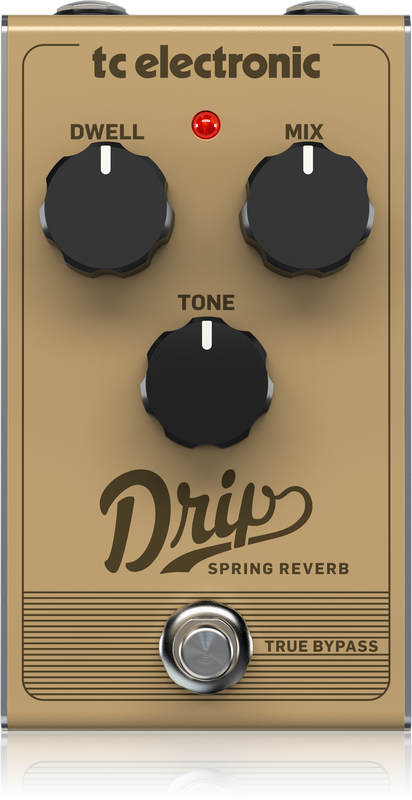
\includegraphics[width=.20\textwidth]{Graphics/EffectPedalExample}
%	 \caption{This figure shows a Drip spring reverb effect pedal by TC Electronics \url{https://www.tcelectronic.com/Categories/Tcelectronic/Guitar/Stompboxes/DRIP-SPRING-REVERB/p/P0CQ2\#googtrans(en|en)}.}
%    \label{fig:EffectPedalExample}
%\end{figure}
%%
%\subsection{The TonePrint Software}
%\label{TonePrintSoftware}
%As previously stated, the exploring of TonePrints start with the TonePrint application available for smartphones and tablets. However, the software is also available for PC and MAC, and the reason for this distinction lies in the difference of how a TonePrint is transferred to its respective pedal. For PC and MAC the user is required to use a cable from the computer to the pedal, but through the tablet and smartphone application, the user also have the option of simply beaming it directly to the pedal. whatever the platform, however, when opening the software the user is introduced to a list selection of different effect pedals, each holding a vast number of TonePrints created by famous guitarists. After selecting an effect pedal from this list, the user is then presented a new list selection of the many guitarist who have created TonePrints for this pedal. When selecting one of the guitarists, and depending on whether the guitarist have created more TonePrints for the same pedal, the user is then presented a bigger view of this specific TonePrint with a description of it and its creator. An example of this is displayed on \autoref{fig:TonePrintAppExample}. Depending on the users' motivation when opening the application first time, they can also choose to browse by artist instead of pedal, if their starting point is to find out what it takes to sound like their favourite artist.
%
%\begin{figure}[H]
%	\centering
%	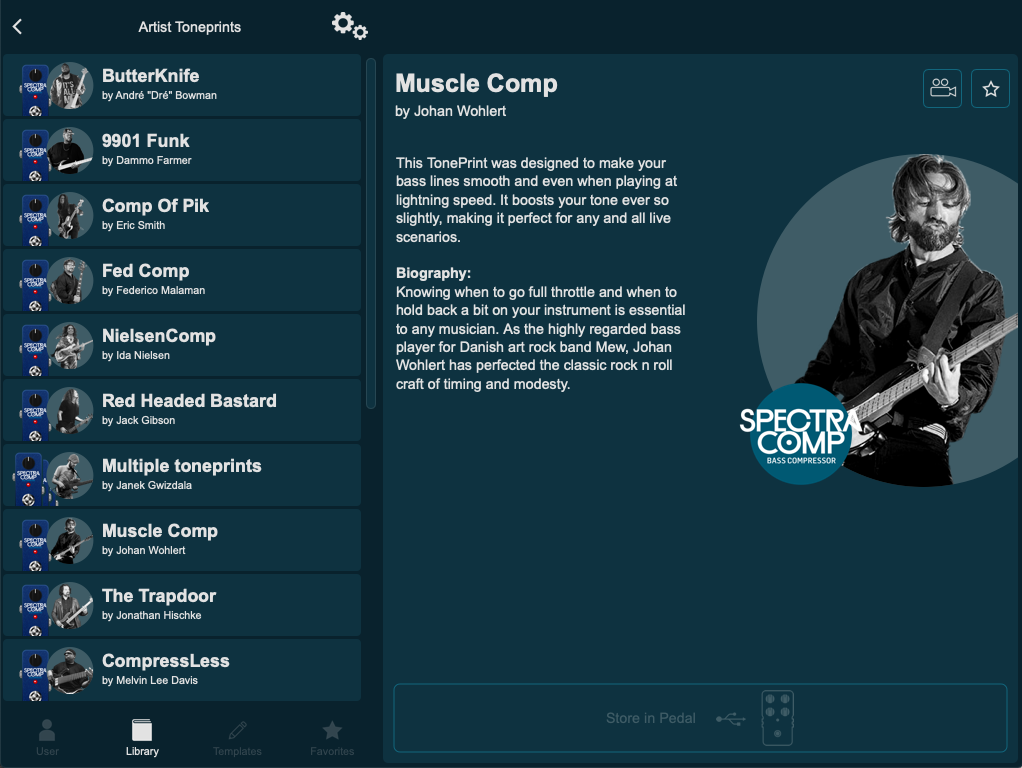
\includegraphics[width=\textwidth]{TonePrintAppExample}
%	\caption{The view in the TonePrint application after selecting an effect pedal and a TonePrint. This example displays a TonePrint created by Johan Wohlert of the danish rock band \textit{Mew}.}
%	\label{fig:TonePrintAppExample}
%\end{figure}
%\noindent

%\begin{itemize}
%	\item Man kan overføre med kabel eller beaming\fxnote{Der skal laves henvisning til appen i sig selv}
%	\item If a user should attempt to transfer a TonePrint of an effect pedal to a completely different unit, it simply wouldn't work.
%	\item Et billede af appen, men hvad skal det billede helt præcist vise? Hvor i appen skal man være?\fxnote{Indsæt billede af appen}
%	\item Brugeren kan også starte med at browse ud fra guitarist i stedet for deal type => Det er ikke til at sige, hvad brugerens motivation er.
%    \item Brug en termologi som ikke kun forståes af musikere og overvej at forklare hvad toneprint er når det nævnes så man ikke skal læse mange linjer før en forklaring kommer.
%    \item overvej at omformulere den øverste "hat" eventuelt fjern den.
%    \item lav en tdligere skillelinje mellem artist og user toneprint.
%\end{itemize}

%\section{What should be in the introduction}
%\label{WhatShouldBeInTheIntroduction}
%
%\begin{itemize}
%	\item A short description of TC Electronic (Just the basics)
%	
%	\begin{itemize}
%		\item TC laver effektpedaler og er kendt på verdensplan
%		\item  A very short description of the principal of TonePrint (A later chapter/section will go more in depth \autoref{TonePrints}
%		\item Something about TC wanting to enable the users to share their UserTonePrints
%	\end{itemize}
%	
%	\item TC wish to include their users in the development of the new sharing platform (Community).
%	
%	\begin{itemize}
%		\item Hvorfor er det generelt en god ide at inddrage brugere til at løse designproblemer?
%		\item Hvad er typiske problemer?
%	\end{itemize}
%	
%	\item Something in general about how communities works and why it's important to include the users in the development of one.	
%	
%	\begin{itemize}
%		\item TC's Koncern community
%		\item Generelt ønske fra brugerne, at de gerne vil have et TonePrint community. - Det kræver kun et besøg på diverse fora for at finde dette ønske
%	\end{itemize}
%
%\end{itemize}


%Processen skal gå fra at TC har ønske om at lave et TonePrint Community. Det vi så skal arbejde hen imod er at finde ud af, hvordan en virksomhed som TC kan foretage brugerinddragelse, og hvordan de specifikt skal gøre det i forhold til dette.